\begin{frame}
\frametitle{Простые алгоритмы аллокации памяти}
\framesubtitle{Постановка задачи}

Чего мы хотим:
\begin{itemize}
  \item<2-> реализовать malloc и free
  \item<3-> чем быстрее тем лучше
  \item<4-> избежать фрагментации памяти, если получится
\end{itemize}
\end{frame}

\begin{frame}
\frametitle{Простые алгоритмы аллокации памяти}
\framesubtitle{Постановка задачи}

\onslide<1->{
Исходные данные - участок памяти:
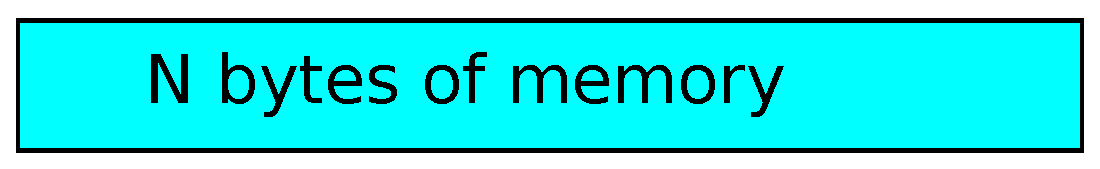
\includegraphics[width=0.9\linewidth]{alloc-basic0}}

\onslide<2->{и, для удобства, какая-то память константного размера:
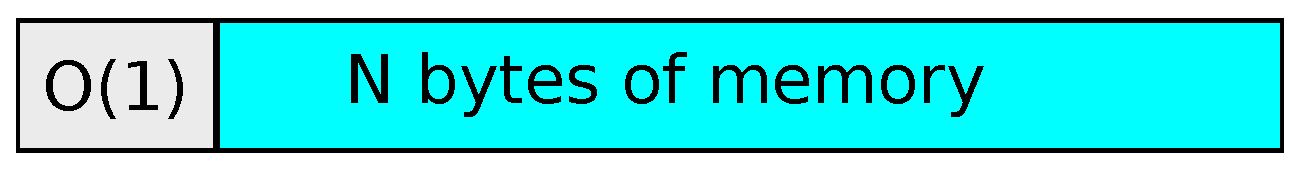
\includegraphics[width=0.9\linewidth]{alloc-basic1}}

\end{frame}

\begin{frame}
\frametitle{Простые алгоритмы аллокации памяти}
\framesubtitle{Аллокация}

Построим в памяти связный список свободных участков:

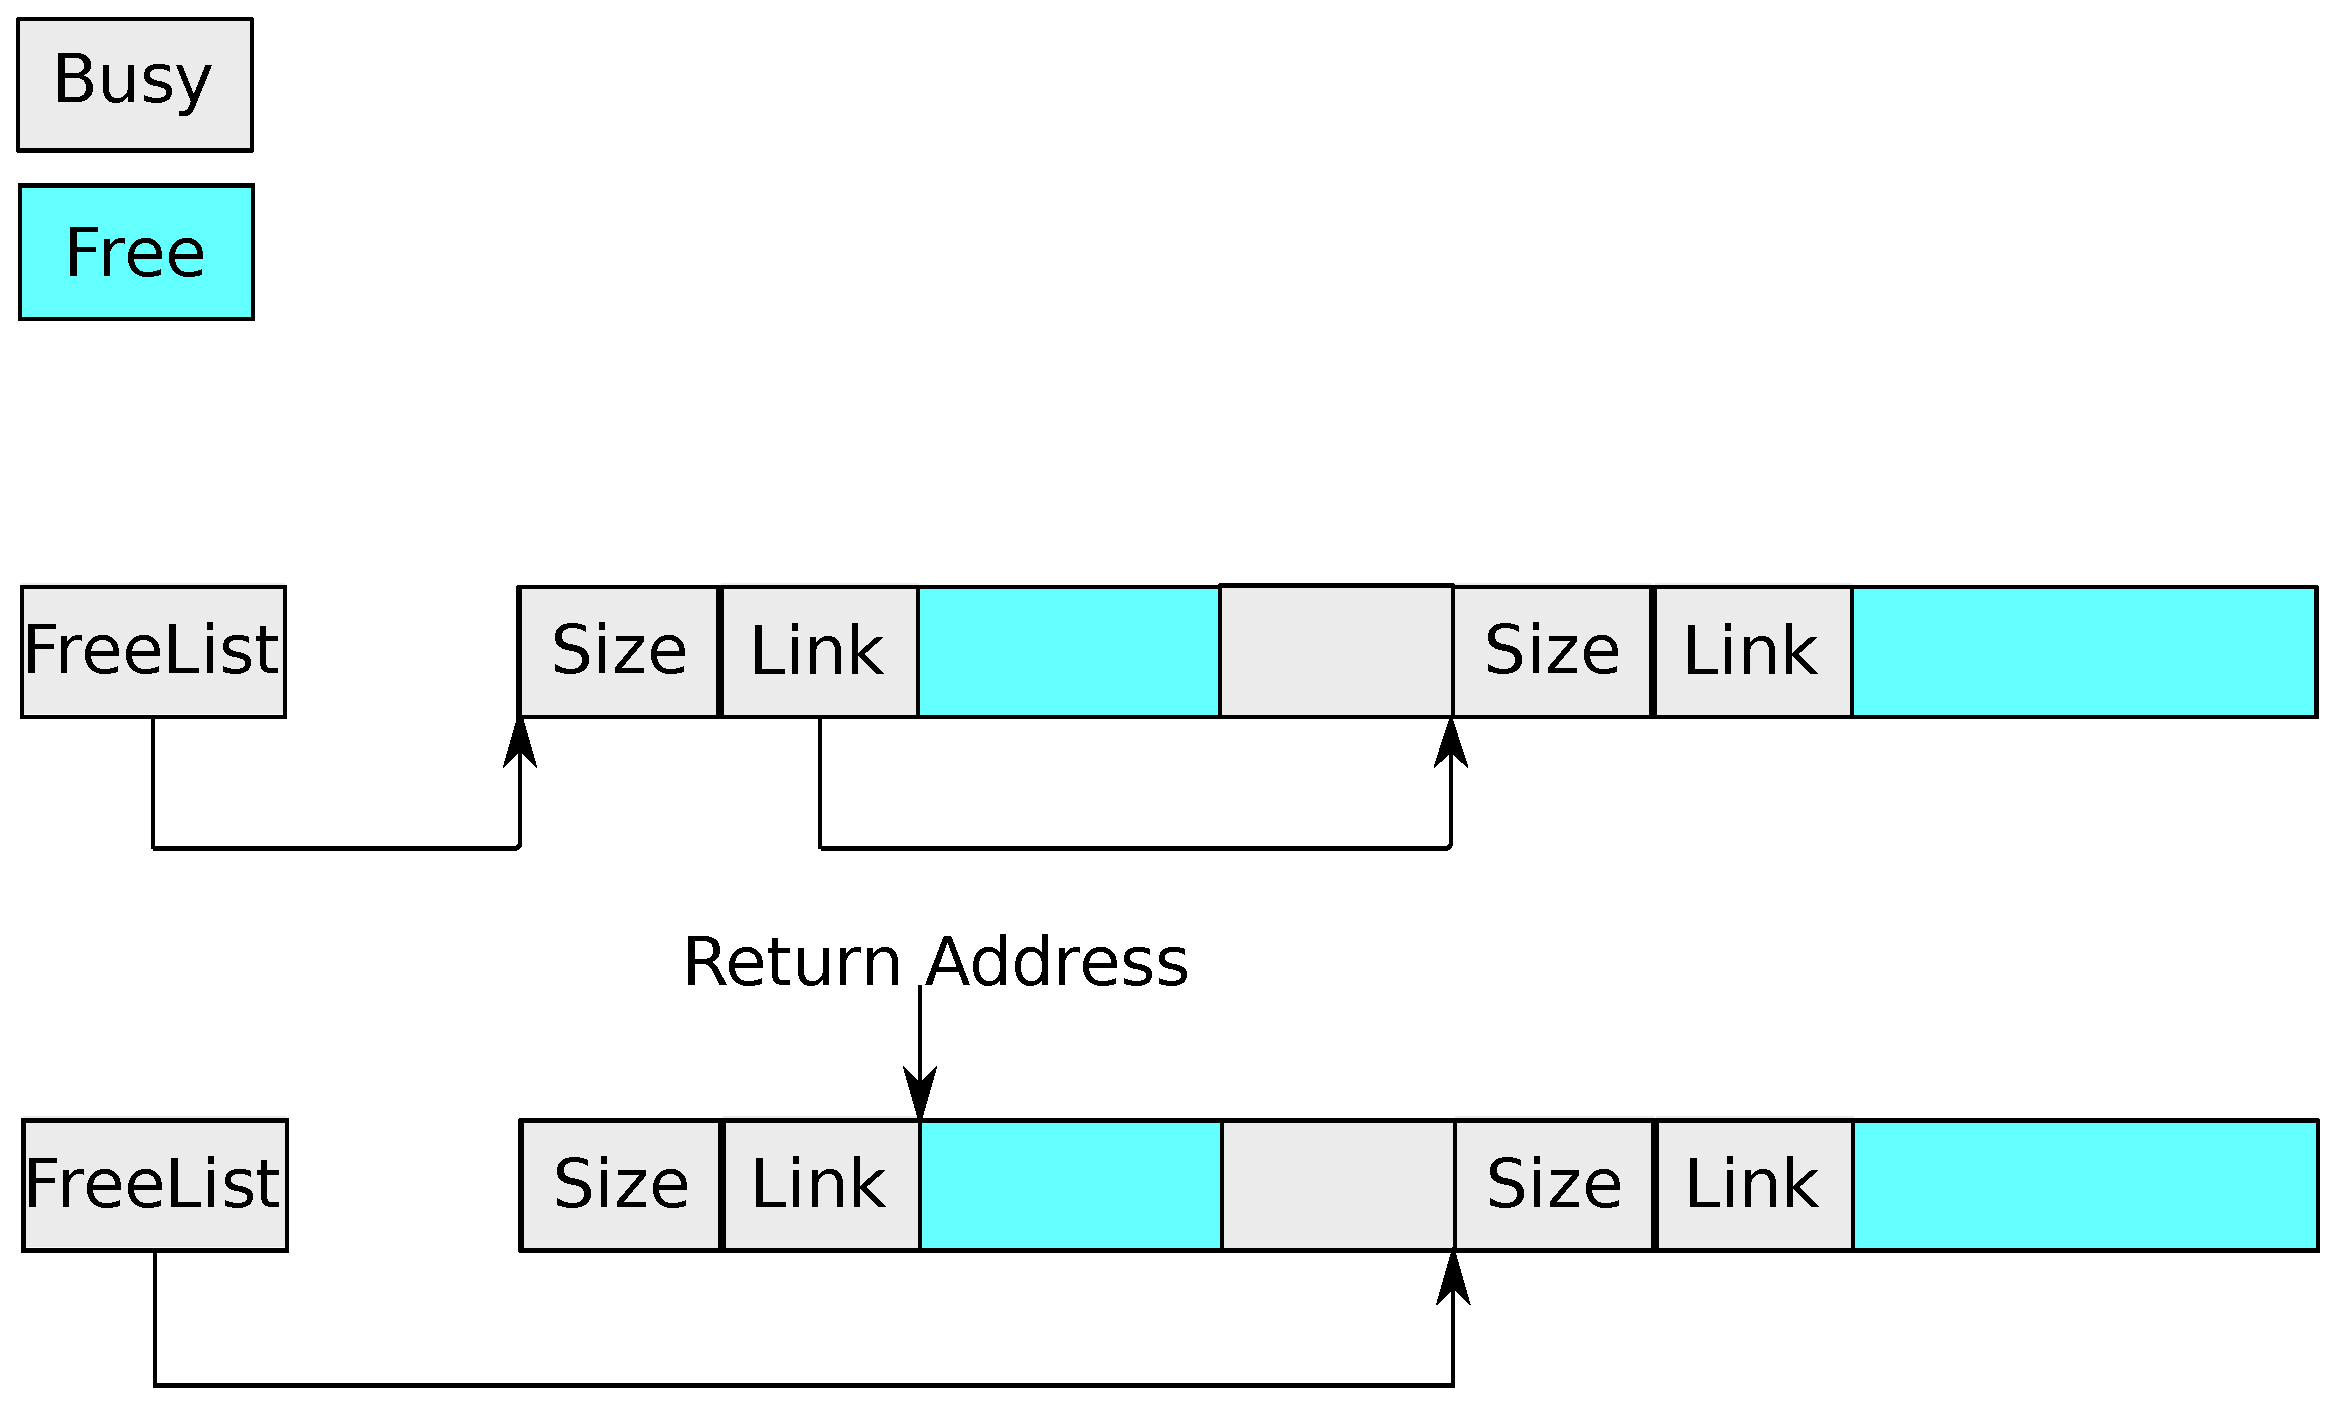
\includegraphics[width=.9\linewidth]{alloc-alloc0}
\end{frame}

\begin{frame}
\frametitle{Простые алгоритмы аллокации памяти}
\framesubtitle{Аллокация}

\onslide<1->{При аллокации проходим список свободных участков и выбираем подходящий.}

\onslide<2->{Как выбрать подходящий?}
\begin{itemize}
  \item<3-> Best Fit - проходим весь список, выбираем наименьший из подходящих
  \item<4-> First Fit - выбираем из списка первый подходящий
\end{itemize}

\onslide<5->{Какая стратегия лучше?}
\begin{enumerate}
  \item<6-> науке это не известно - разные приложения используют память по разному
  \item<7-> зачастую First Fit лучше - не нужно проходить весь список при прочих равных (неизвестных)
  \item<8-> простые алгоритмы редко используются на практике - есть лучшие подходы
\end{enumerate}
\end{frame}

\begin{frame}
\frametitle{Простые алгоритмы аллокации памяти}
\framesubtitle{Аллокация}

Почему бы пользователю не запоминать размер аллоцируемого блока? В простых случаях это будет работать хорошо:
\begin{itemize}
  \item часто размер известен в момент компиляции (sizeof(...))
  \item часто размер объекта вам нужен сам по себе - можно избежать дублирования
  \item пользователь сам определяет, где и как хранить размер
\end{itemize}
\end{frame}

\begin{frame}
\frametitle{Простые алгоритмы аллокации памяти}
\framesubtitle{Аллокация}

Однако в нашем случае это не будет работать - аллоцированный блок может быть больше запрошенного:

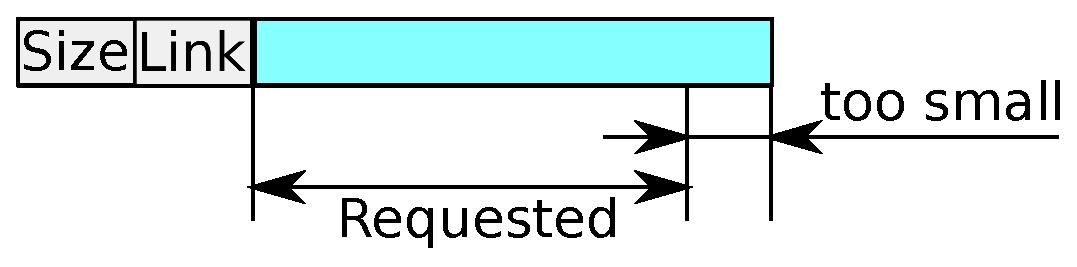
\includegraphics[width=.9\linewidth]{alloc-alloc1}
\end{frame}

\begin{frame}
\frametitle{Простые алгоритмы аллокации памяти}
\framesubtitle{Освобождение}

Функция освобождения принимает указатель как аргумент, нам так же нужен размер участка памяти:

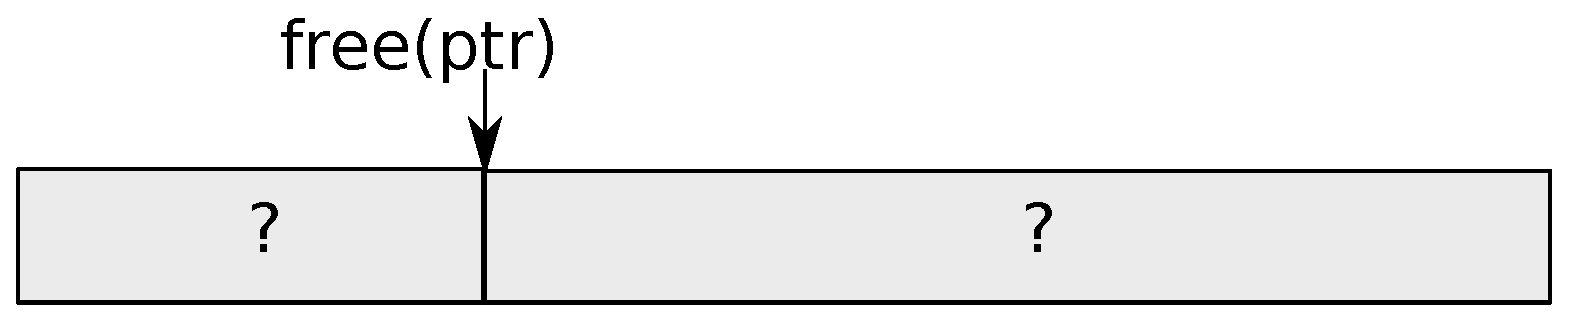
\includegraphics[width=.9\linewidth]{alloc-free0}

\onslide<2->{
\includegraphics[width=.9\linewidth]{alloc-free1}
}

\end{frame}

\begin{frame}
\frametitle{Простые алгоритмы аллокации памяти}
\framesubtitle{Освобождение}

Самый простой вариант, просто добавить элемент в список (начало или конец):

\includegraphics[width=.9\linewidth]{alloc-free2}

\includegraphics[width=.9\linewidth]{alloc-free3}

\end{frame}

\begin{frame}
\frametitle{Простые алгоритмы аллокации памяти}
\framesubtitle{Освобождение}

Рано или поздно это приведет к проблеме:

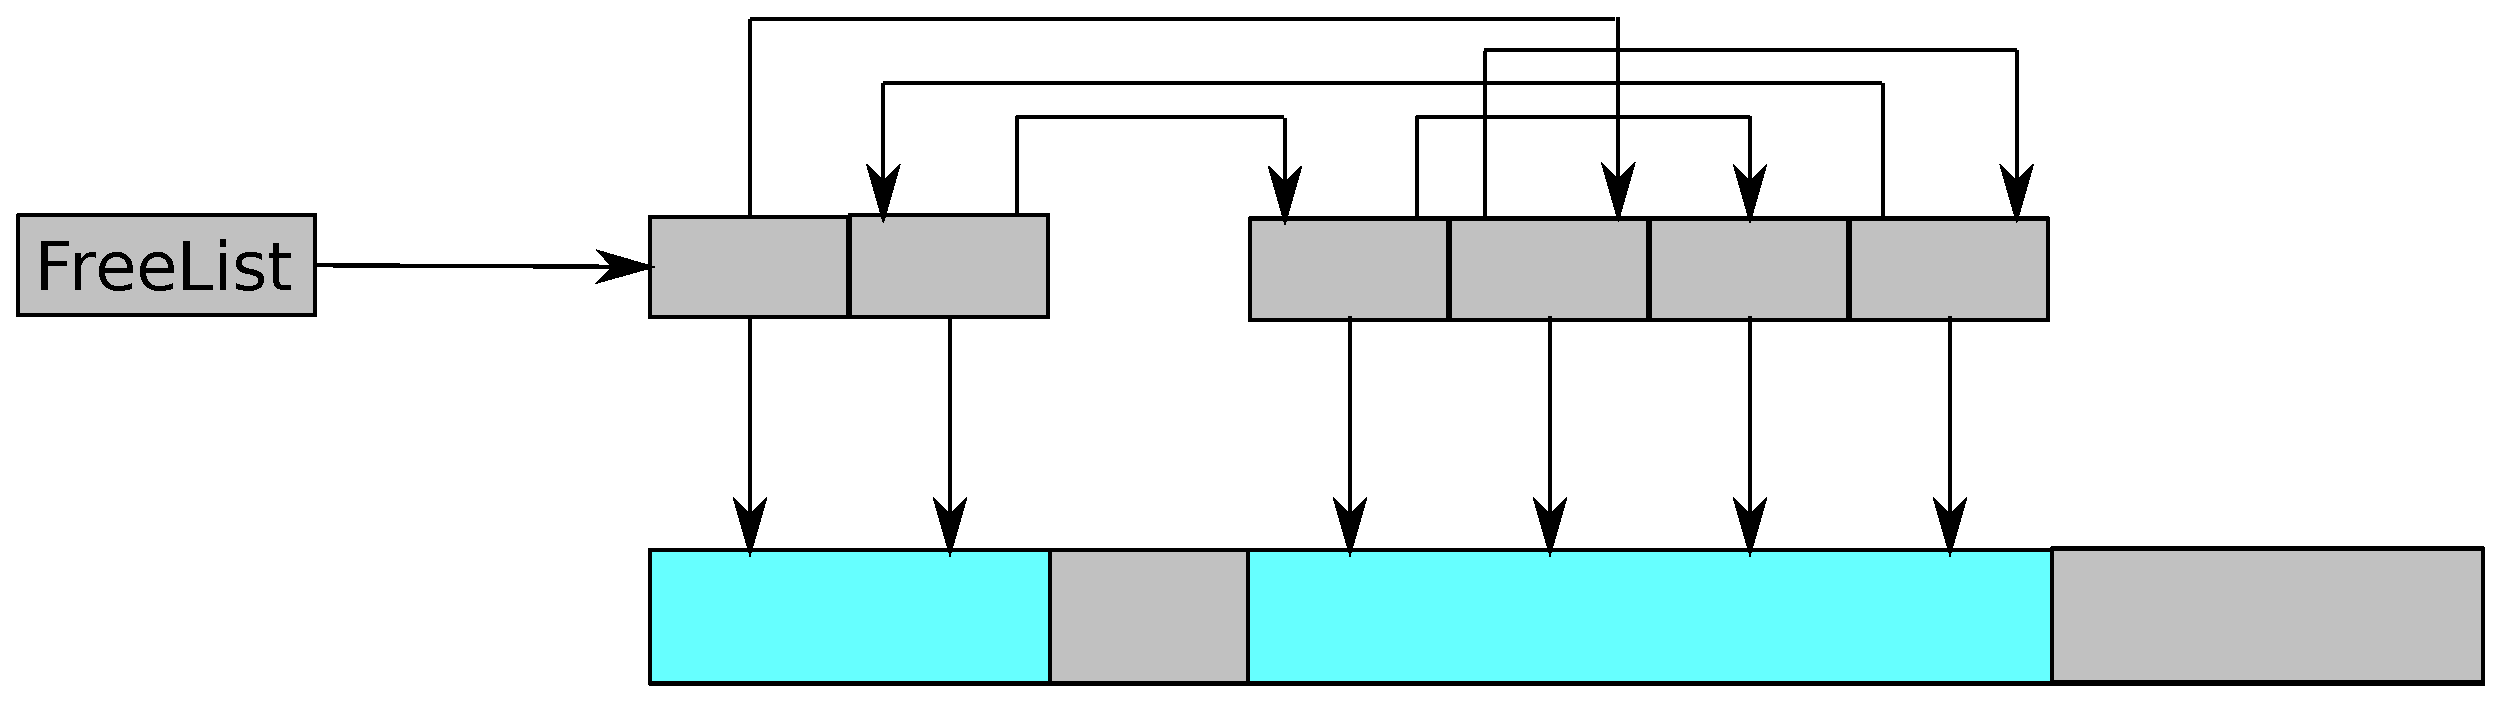
\includegraphics[width=.9\linewidth]{alloc-free4}

\end{frame}

\begin{frame}
\frametitle{Простые алгоритмы аллокации памяти}
\framesubtitle{Освобождение}

При освобождении необходимо объединять соседние свободные блоки:
\begin{itemize}
  \item<2-> чтобы не фрагментировать память, иначе мы не сможем аллоцировать большие участки памяти
  \item<3-> чтобы список свободных блоков не разрастался - плохо влияет на время аллокации памяти
\end{itemize}

\end{frame}

\begin{frame}
\frametitle{Простые алгоритмы аллокации памяти}
\framesubtitle{Освобождение}

Как объединять соседние свободные блоки:
\begin{itemize}
  \item<2-> мы можем поддерживать список отсортированным по адресу (классический версия malloc в UNIX, aka SLOB, описана в The C Programming Language)
  \item<3-> вместо списка можно использовать дерево - жертвуем памятью в обмен на производительность
  \item<4-> можно использовать Border Tags (авторство приписывают Кнуту, но идея очень очевидная)
\end{itemize}

\end{frame}

\begin{frame}
\frametitle{Простые алгоритмы аллокации памяти}
\framesubtitle{Освобождение}

Мы уже храним служебную информацию в начале блока, давайте добавим еще и в конец:
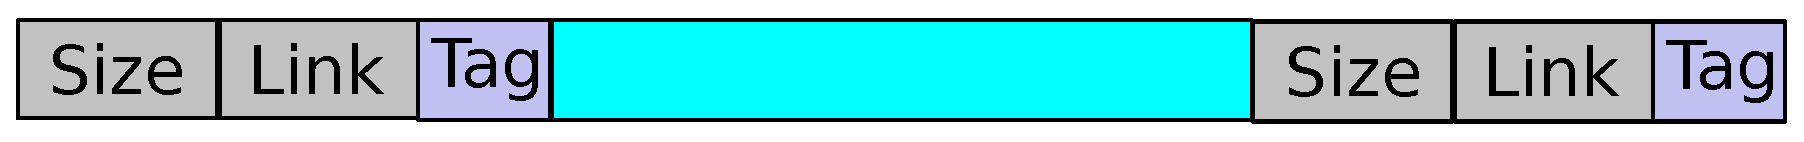
\includegraphics[width=.9\linewidth]{alloc-tag0}

\begin{itemize}
  \item<2-> TAG - индикатор свободности/занятости блока (это и есть Border Tag)
  \item<3-> Link-и в начале и в конце можно использовать как ссылки на следующий и ссылки на предыдущий блоки (просто для экономии памяти)
\end{itemize}

\end{frame}

\begin{frame}
\frametitle{Простые алгоритмы аллокации памяти}
\framesubtitle{Освобождение}

Мы знаем где находится Border Tag предыдущего (следующего) блока и можем легко
проверять свободность/занятость:
\includegraphics[width=.9\linewidth]{alloc-tag1}

\onslide<2->{
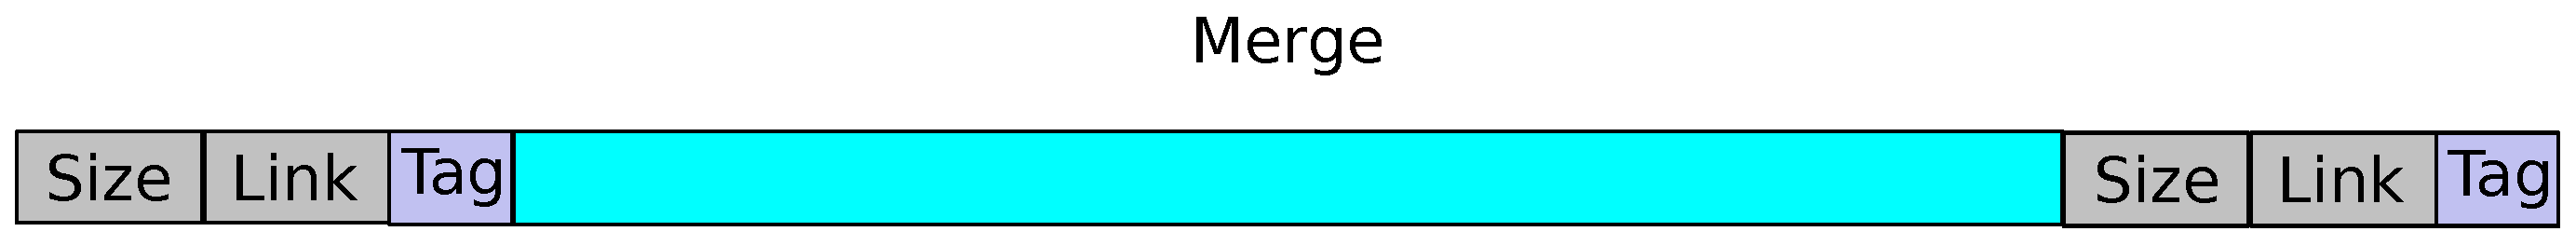
\includegraphics[width=.9\linewidth]{alloc-tag2}

При объединении сразу трех блоков нужно удалить один из двусвязного спика - O(1).
}

\end{frame}
